\documentclass{RITA}
\usepackage{amssymb,amsfonts,mathtools,float,subfigure,url,times,graphicx,pslatex,multicol,footmisc,cite}
\usepackage{titlesec}

% Equation terms definition
\newcommand{\route}[1]{\ensuremath{P_#1}}	%route for driver 'i'
\newcommand{\optRoute}[1]{\ensuremath{P_#1^*}}	%optimal route for driver 'i'

\newcommand{\travTime}{\ensuremath{t_j}} 	%travel time on link 'j'
\newcommand{\fftt}{\ensuremath{f_j}} 		%free-flow travel time of link 'j'
\newcommand{\linkCap}{\ensuremath{c_j}}		%capacity of link 'j'
\newcommand{\veh}{\ensuremath{v}}		%number of vehicles

\newcommand{\ett}[1]{\ensuremath{t'_{#1}}}		%estimated travel time for agent 'i'
\newcommand{\expVeh}[1]{\ensuremath{\tilde{\veh}_{\optRoute{#1}}}}		%estimated number of vehicles

\newcommand{\att}[1]{\ensuremath{\hat{t}_{#1}}}		%actual travel time for driver 'i' on route P

\newcommand{\reward}[1][]{\ensuremath{R_#1}}	%reward

\newcommand{\congRoads}{\ensuremath{C}}		%the set of congested roads
\newcommand{\numCong}{\ensuremath{n}}		%number of congested roads
\newcommand{\overLoadFactor}{\ensuremath{o}}	%overload factor - measures severity of congestions

\newcommand{\numepis}{\ensuremath{\eta}}	%the number of episodes

\title{Independent learners in abstract traffic scenarios}

\author{
  Anderson Rocha Tavares\footnote{Instituto de Inform\'atica, UFRGS, Caixa Postal~15064\\
  \texttt{\{artavares,bazzan@inf.ufrgs.br\}}}
  \and Ana Lucia Cetertich Bazzan\footnotemark[1]
}

\RITAvolume{?}
\RITAnumber{?}
\RITAyear{2012}
     

\hyphenation{sev-er-ral learn-ing meth-ods be-hav-ior a-vail-a-ble pa-ram-e-ters dif-fer-ent}

\begin{document}

\maketitle

\begin{abstract}
In transportation systems, drivers usually choose their routes in an uncoordinated way. In general, this leads to poor global and individual performance regarding travel times and road network load balance. This work presents a reinforcement learning based approach for route choice which relies solely on drivers' experience to guide their decisions. 
There is no coordinated learning mechanism, thus driver agents are independent learners. Our approach is tested in two abstract traffic scenarios and it is compared to other route choice methods. 
Experimental results show that drivers learn routes in complex scenarios. Moreover, the approach outperforms the compared route choice methods regarding drivers' travel time. Also, satisfactory performance is achieved regarding road network load balance. 
The simplicity, realistic assumptions and performance of the proposed approach suggest that it is a feasible candidate for implementation in navigation systems for guiding drivers decisions regarding route choice.
\end{abstract}
% \index{annotation pipeline}
% \index{\emph{A. thaliana}}
% \index{Keywords in swissprot}

%\category{I.2.11}{Artificial Intelligence}{Distributed Artificial Intelligence}[Multiagent Systems]

%\terms{Algorithms}

%\keywords{Multiagent reinforcement learning, multiagent systems, traffic assignment}

\section{Introduction}
\label{sec:intro}

Traffic and mobility present challenging issues to authorities, traffic engineers and researchers. To deal with the increasing traffic demand, techniques and methods to optimize the use of the existing road traffic networks are attractive since they do not include expensive and environmental-impacting changes on the infrastructure.

In a commuting scenario, it is reasonable to assume that drivers choose their routes independently from one another and that previous experience is taken into account when they are choosing a route. Daily commuters usually have an expectation about the time needed to arrive on their destinations and, if a driver reaches its destination within that expectation, its travel time can be considered  reasonable. In a commuting scenario, drivers strive to minimize their travel times. At the same time, there is a global cost function that rates the whole system's behavior, such as the distribution of vehicles in proportion to the capacity of each road. Multiagent systems such as this commuting scenario are called collectives. The local and global goals can be highly conflicting and there is no general approach to tackle this complex question of collectives, as shown by Tumer and Wolpert \cite{Tumer&Wolpert2004}.

Traffic assignment concerns the allocation of a given set of drivers to specific routes, satisfying the demand between origins and destinations in transportation networks. In this work, traffic assignment is modeled as a reinforcement learning problem. Agents make decisions using only their own experience, which is gained through interaction with the environment. The environment is a road network that abstracts some real-world characteristics such as vehicle movement along the roads, allowing us to focus on the main subject which is the choice of one route among the ones available for each driver.

The remainder of this document is organized as follows: Section \ref{sec:concepts} presents basic concepts about traffic network modeling and reinforcement learning that are used throughout this paper. Section \ref{sec:related} presents and discusses related work. Section \ref{sec:proposal} presents the reinforcement learning approach for route choice that is tested in the scenarios described in Section \ref{sec:scenario}. Results are presented and discussed in Section \ref{sec:results}. Finally, Section \ref{sec:conclusions} concludes the paper and presents opportunities for further investigation.

\section{Background}
\label{sec:concepts}
\subsection{Road traffic network modeling}

A road network can be modeled as a graph, with a set of nodes that represents the intersections, and links among these nodes, which represent the road sections. The weight of a link represents a form of cost associated with the link. For instance, the cost can be the travel time, fuel spent or length. 

The road network contains origins and destinations that are subsets of the set of nodes. A driver's trip consists of a set of links, forming a route between his origin and destination nodes (OD pair). A commuting scenario consists of repeated trips, such as drivers going from home to work approximately in the same hour of the day during the workdays.

Drivers travelling through the road network generate traffic flow. Traffic assignment methods need a suitable cost function that relates traffic flow and link's attributes (capacity, free-flow travel time). % However, a simplified form that relates attributes of a  given link and traffic flow only on that link can be used, although with some loss of realism.
One of the most common function of this type is shown Eq. \eqref{eq:tt} \cite[Section~10.1.3]{Ortuzar&Willumsen2001}.

\begin{equation}
\label{eq:tt}
\travTime(\veh) = \fftt[1 + \tau \left(\frac{\veh}{\linkCap}\right)^\beta]
\end{equation}

In this function, $\travTime$ is the travel time on link $j$ applied to the number of vehicles ($\veh$), $\linkCap$ is the link's capacity, $\fftt$ is the free-flow travel time on link $j$ and $\tau$ and $\beta$ are calibration parameters. This is the travel time function used throughout the present work.

\subsection{Reinforcement Learning}
\label{sec:rl}
Reinforcement learning (RL) deals with the problem of making an agent learn a behavior by interacting with the environment. Usually, a reinforcement learning problem is modeled as a Markov decision process (MDP), which consists of a discrete set of environment states $(S)$, a discrete set of actions $(A)$, a state transition function ($T: S \times A \to \Pi(S))$, where $\Pi(S)$ is a probability distribution over $S$ and a reward function $(R: S \times A \to \mathbb{R})$. %$T(s, a, s')$ means the probability to go from state $s$ to $s'$ after performing action $a$ in $s$.

The agent interacts with the environment following a policy $\pi$ and tries to learn the optimal policy $\pi^*$ that maps the current environment state $s \in S$ to an action $a \in A$ in a way that the future reward is maximized. At each state, the agent must select an action $a$ according to a strategy that balances exploration (gain of knowledge) and exploitation (use of knowledge). One possible strategy is $\epsilon$-greedy, that consists in choosing a random action (exploration) with probability $\epsilon$ or choosing the best action (exploitation) with probability $1 - \epsilon$. In the beginning, $\epsilon$ starts with a high value (high exploration) and decreases with time, leading to high exploitation in the end.

Q-learning is an algorithm that converges towards the optimal policy, given certain conditions \cite{Watkins&Dayan1992}. Its update rule is shown in Eq. \eqref{eq:qlearning}, where $<s,a,s',R>$ is an experience tuple, meaning that the agent performed action $a$ in state $s$, reaching state $s'$, receiving reward $R$. Action $a'$ is one that can be taken on $s'$, $\alpha \in [0:1]$ is the learning rate, and $\gamma \in [0:1]$ is the discount factor. $Q(s,a)$ is an entry indexed by state $s$ and action $a$ in the Q-table, which stores the values (called Q-values) of state-action pairs. The Q-value is the expected discounted reward for executing action $a$ at state $s$ and following the policy $\pi$ thereafter. For a complete description of Q-learning, the reader may refer to \cite{Watkins&Dayan1992}.

\begin{equation}
\label{eq:qlearning}
Q(s,a) = (1 - \alpha) Q(s,a) + \alpha (R + \gamma \max_{\substack{a'}}(Q(s',a')))
\end{equation}

%For the next sections it will be assumed that the reader is familiar with Q-learning. For more information about Q-learning, the reader may refer to \cite{Watkins&Dayan1992}.

\subsection{Independent learners} 
%Traffic scenarios are associated with the class of non-cooperative multiagent systems. %In traffic, drivers can be regarded as agents that use the traffic network resources. 
Multiagent reinforcement learning (MARL) can be divided in two classes: independent learners (ILs), in which agents ignore the existence of other agents, and joint action learners (JALs), in which agents learn the value of their own actions combined with other agents' actions via integration of RL with coordination learning methods \cite{Claus&Boutilier1998}. 

In complex scenarios such as transportation systems, there is a large number of agents, making the modeling of JALs unfeasible, as remarked by Bazzan in \cite{Bazzan2009}. On the other hand, when agents are modeled as ILs, the convergence properties of Q-learning become invalid, as the environment is nonstationary. Also, it is remarked by Littman \cite{Littman1994} that training adaptive agents without considering other agents adaptation is not mathematically justified and it is prone to reaching a local maximum where agents quickly stop learning. Despite this, some researchers achieved satisfactory results with this approach \cite{Littman1994}. Therefore, in the present work, agents are modeled as ILs.

It must be remarked however that for an independent learner agent, the other agents learning and changing their behavior is understood as a change of the environment dynamics.  %, because modeling agents as JALs leads to scalability problems, as agents must consider every other agents' actions. 

One example of successful application of independent learners can be found in \cite{Tesauro1994}, where the author presents an automated player that uses the TD($\lambda$) reinforcement learning algorithm \cite{Sutton1988} to teach itself to play backgammon. From zero knowledge in the beginning of learning, the automated player learns to play at a strong intermediate level. The automated player reaches strong master level if some prior knowledge is programmed in it. 

Another example of successful application of independent learners can be found in \cite{Crites&Barto1998}, where the authors program each member of an elevator car controller team as an independent learner. Results show that the presented approach surpasses the best heuristic elevator control algorithms of that time.

%A multiagent system can be understood as group of agents that interact with each other besides perceiving and acting in the environment they are situated. The behavior of these agents can be designed a priori. In some scenarios this is a difficult task or this pre-programmed behavior is undesired, so that the adoption of learning (or adapting) agents is a feasible alternative \cite{Busoniu+2008smc}.



\section{Related work}
\label{sec:related}

%In traffic engineering, \cite{Bazzan&Kluegl2007} remarks that agent-based simulation is a suitable approach, as agents can be modeled to deal with incomplete information and adapt to dynamic environments. Application of intelligent agent architectures to route choice is present on a number of publications. Next, some works based on this agent-based approach are reviewed.

%Several works, such as \cite{Bazzan+2000icmas,Chmura&Pitz2007,Kluegl&Bazzan2004}, use abstract scenarios, most of the times inspired by congestion or minority games. On these scenarios, agents have to decide between two routes and receive a reward based on the occupancy of the chosen route. This process is repeated and there is a learning or adaptation mechanism that guides the next choice based on previous rewards.

%With this process, a Pareto-efficient distribution or the Wardrop's equilibrium \cite{Wardrop1952} may be reached. In this condition, no agent can reduce its costs by switching routes without rising costs for other agents. 

Traffic assignment problems can be addressed by several approaches, many of them considering abstract traffic scenarios. Two-route scenarios are studied in \cite{Bazzan+2000icmas,Kluegl&Bazzan2004jasss}. The former work assesses the effect of different strategies for binary route choice. The latter presents a model where commuters' behavior is based on evolving heuristics and also performs experiments regarding route choice with a forecast: a traffic control system perceives drivers' decisions and returns a forecast. Then drivers have to decide the actual route selection. %The third uses a reinforcement learning scheme to reproduce human decision-making in a corresponding experimental study.

Each one of these works assessed relevant aspects of the agents' decision-making process, even though only binary route choice scenarios were studied. The interest of the present work is to evaluate a route choice approach in more complex scenarios, with several routes.

This kind of complex scenario was investigated by Bazzan and Kl\"ugl \cite{Bazzan&Kluegl2008}, where the effect of real time information on drivers' route replanning is assessed. The work includes studies with adaptive traffic lights. In the most successful en-route replanning strategy presented in that work, the authors assume that the entire network occupancy is known by the drivers. This assumption was needed for assessing the effects of re-routing, although the availability of real time information of the entire network for all the drivers is  unrealistic.

The use of information to aid drivers decisions is also studied by Yamashita and Kurumatani in \cite{Yamashita&Kurumatani2009}, where authors present a route information sharing system. In this system, drivers send their current position, destination and route to a server that estimates traffic conditions in the future and returns this estimation for the drivers. Upon receipt of the estimation, drivers decide whether to recalculate their routes or not. However, the proposed approach relies on a centralized route information server and requires a communication infrastructure that is not yet available.

%More recently, Galib and Moser \cite{Galib&Moser2011} proposed a modified version of the minority game for use in a complex scenario with several available routes. 
The problem of traffic assignment can also be tackled by the evolutionary version of the minority game \cite{Challet&Zhang1997} such as in the work of Galib and Moser in \cite{Galib&Moser2011}. In evolutionary games, it is assumed that players (or agents) have bounded rationality and use inductive reasoning to make their decisions. This is suitable to the transportation domain as humans do have bounded rationality and inductive reasoning is used in human decision-making process, as remarked by Arthur \cite{Arthur1994}.

In the minority game, an odd number of player agents must choose between two options. At each round, agents on the minority side win and receive a reward. Agents keep a memory of the history of winning options and use this information to act in the next round. Each player agent has a finite set of strategies that map the history of winning options to an option to be chosen in the next round. Each strategy is scored according to the number of times it went correct. Player agents use the strategy with the highest score to act in the next round.

Regarding traffic assignment, the minority game can only be used in two-route choice scenarios as it is a two-alternative game. To overcome this limitation, Galib and Moser \cite{Galib&Moser2011} proposed a modified version of the minority game for a complex scenario with several available routes. In this modified version, for each road network link, each driver agent has a finite set of strategies that predict the link's occupancy given the occupancy history on the past trips. Each strategy is scored according to the actual link's occupancy and the total travel time of the driver agent. Using the proposed approach, drivers achieve reasonable (within expectation) travel times and distribute themselves over the road network in a way that few links get overused. In the proposed approach, driver agents have historical occupancy data of all links of the road network. For a driver, having historical information of the links it used is a reasonable assumption, but having historical information of all links on the network is unrealistic. The approach proposed on the present work is compared with the modified minority game of \cite{Galib&Moser2011}, as shown in Section \ref{sec:comparison}. 

%TODO cut other IL works???%%% Prior to the present work, independent learning agents were studied in cooperative repeated games \cite{Claus&Boutilier1998,Tan1993,Sen+1994}. The present study is an application of the independent learners concept in a competitive multi-agent system as agents compete for a resource (the road network). Decisions on this route choice scenario are sequential, making this a more complex scenario.

Learning-based models for route choice appear in \cite{Chmura&Pitz2007,Ben-Elia&Shiftan2010}. In \cite{Chmura&Pitz2007}, the authors test human behavior in the minority game. In the experiments, human subjects must choose repeatedly between two routes. In \cite{Ben-Elia&Shiftan2010}, real-time traffic information is given to human subjects and they must choose between two routes. The authors conclude that both experience and information play a role in the choices made by the subjects.

Both works are focused on presenting reinforcement based models for human behavior estimation, rather than proposing a new approach for improving the route choice process in a scenario with several available routes. 

Such approach can be found in \cite{Tavares&Bazzan2012}, where we have modeled traffic assignment as a MDP with no states. The actions set comprises the selection of network links and the reward function is based on the link's travel time weighted by a factor that takes the whole route travel time into account. The performance of the proposed approach is assessed in the same scenario studied by Galib and Moser \cite{Galib&Moser2011} and satisfactory results are obtained regarding travel times (on average, drivers achieve travel times within expectation) and roads occupancy (only few roads get overloaded). 

In the present work, the traffic assignment problem is modeled as a MDP with states and the reward function is simplified taking into account only the travel time in the chosen link. Also, in relation to \cite{Tavares&Bazzan2012}, new metrics for road congestion evaluation are proposed and the RL-based approach is compared with more route choice strategies. %The present work also studies the RL approach in a 6x6 grid scenario, that resembles some real-world features, bringing the RL approach closer to reality.

To the best of our knowledge, a reinforcement learning based approach for the route choice process with arbitrary number of routes was found only in \cite{Tavares&Bazzan2012}. In other works, either researchers present other approaches (such as the use of real-time information or minority games) for the problem, or reinforcement based schemes are used to try to reproduce human behavior in two-route scenarios.

\section{Proposed approach}
\label{sec:proposal}

\subsection{Reinforcement learning for route choice}

The MDP model (as seen in Section \ref{sec:rl}) for this problem is as follows: the states are the nodes of the  road network. The set of actions comprises the selection of the outbound links from the nodes of the network. Not every link will be available for an agent to choose, as it depends on which node of the network it is and whether the link belongs to a possible route of the agent. The reward function is given by Eq. \eqref{eq:reward}, where $\travTime$ is the travel time function given in Eq. \eqref{eq:tt} applied to the number of vehicles ($\veh_j$) on link $j$. The reward decreases as travel time increases, thus drivers will strive to minimize their individual travel times.

\begin{equation}
\label{eq:reward}
\reward{} = - \travTime(\veh_j)
\end{equation}

\subsection{Building the route}

Each learning episode is a trip that drivers do departing from their origins and driving to their destinations. One execution consists of the repetition of $\numepis$ learning episodes. At the end of an execution, the performance metrics are assessed. Those metrics are discussed in Section \ref{sec:gridDescription} and \ref{sec:nineODDescription}.

\subsubsection{Initialization:}
At the beginning of the execution, OD pairs are randomly assigned to each driver. The desired initial and final values for the drivers' exploration coefficient ($\epsilon_0$ and $\epsilon_f$, respectively) are assigned and $\epsilon$ receives $\epsilon_0$. The value of $\epsilon_0$ must be high (close to 1) and $\epsilon_f$ must be small so that drivers will initially explore to gain knowledge about the road network and exploit it in the final episodes. Also, the value of the multiplicative factor (0 $< \lambda <$ 1) is calculated via Eq. \eqref{eq:lambda}, where $\numepis$ is the number of learning episodes. This factor is used to decrease $\epsilon$ at the end of each episode (step 6 in Fig. \ref{fig:flowchart}).

\begin{equation}
\label{eq:lambda}
\lambda = \sqrt[\numepis]{\frac{\epsilon_f}{\epsilon_0}}
\end{equation}

\subsubsection{Execution:}

In each episode, each driver follows the steps shown in Fig. \ref{fig:flowchart}.

\begin{figure}[ht]
    \centerline{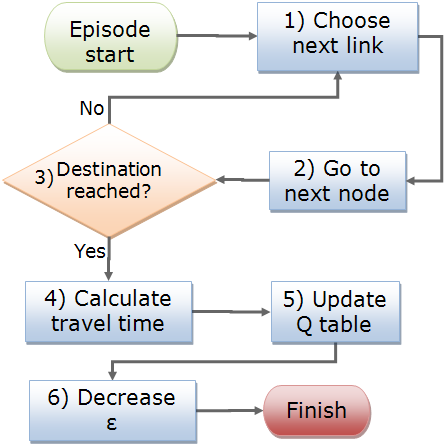
\includegraphics[width=7cm]{img/flowchart3.png}}
    \caption{RL for route choice flowchart}
    \label{fig:flowchart}
\end{figure}

At episode start, all drivers are placed in their origins. At step 1, the driver chooses an outbound link to traverse according to the $\epsilon$-greedy action selection strategy (random action with probability $\epsilon$, best known action with probability $1 - \epsilon$). At step 2, the destination node of the chosen link is reached. At step 3, the driver tests whether the node reached is its final destination. If so, the trip ends. Otherwise steps 1 to 3 are repeated. At step 4, each driver $i$ calculates its travel time $\att{\route{i}}$ experienced on its route $\route{i}$, given by Eq. \eqref{eq:att}. In this equation, $\travTime$ is the travel time function given in Eq. \eqref{eq:tt} applied to the number of vehicles on link $j$ ($\veh_j$). Then, at step 5, drivers update their Q-tables according to Eq. \eqref{eq:qlearning}. Finally, at step 6, the exploration coefficient $\epsilon$ is decreased by the multiplicative factor $\lambda$.

\begin{equation}
\label{eq:att}
\att{\route{i}} = \sum_{j \in \route{i}} \travTime(\veh_j)
\end{equation}



\section{Scenarios and evaluation}
\label{sec:scenario}
In the present work, two scenarios are studied. The first scenario is a 6x6 grid (Fig. \ref{fig:6x6grid}), already investigated in \cite{Bazzan+2007alag,Bazzan+2008alamas} in which no RL mechanism was employed. In the present work, two questions are addressed in the 6x6 grid scenario:

\begin{enumerate}
  \item Can drivers learn the routes from origins to destinations without prior knowledge in a nonstationary scenario? As routes are not pre-computed, drivers need to learn how to travel from their origins to their destinations.
  \item How sensitive is the RL approach for route choice regarding the Q-learning parameters? In this question, we want to assess the influence of the learning rate and the discount rate for future rewards on overall drivers' performance.
\end{enumerate}

The second scenario (Fig. \ref{fig:roadnetwork}) has nine possible origin-destination pairs. It is less complex than the 6x6 grid as the number of possible routes between origins and destinations is lower and it is not possible to build routes with loops as there are no returning links. This scenario was already studied in \cite{Tavares&Bazzan2012,Galib&Moser2011}. The present work compares the RL approach against three methods for route choice in the nine OD pairs scenario.

\subsection{6x6 grid}
\label{sec:gridDescription}
This abstract scenario contains 36 nodes connected by 60 links, as shown in Fig. \ref{fig:6x6grid}. All links are one-way. From the point of view of route choice, this is a complex scenario as the number of possible routes between two locations is high and it is possible to build routes with loops, as there is no pre-computation of shortest paths from origins to destinations. For this reason, there is a limit in the number of steps in each episode: if a driver does not find a path to its destination in 500 steps, the trip is aborted.

Prior experimentation has shown that the limit of 500 steps per episode yields a good trade-off between drivers' learning and execution time. That is, with a lower limit, drivers tend to get stuck for a higher number of episodes until finding a route between their origins and destinations. On the other hand, with a higher limit, drivers can take too much time to find a route.

\begin{figure}[ht]
    \centerline{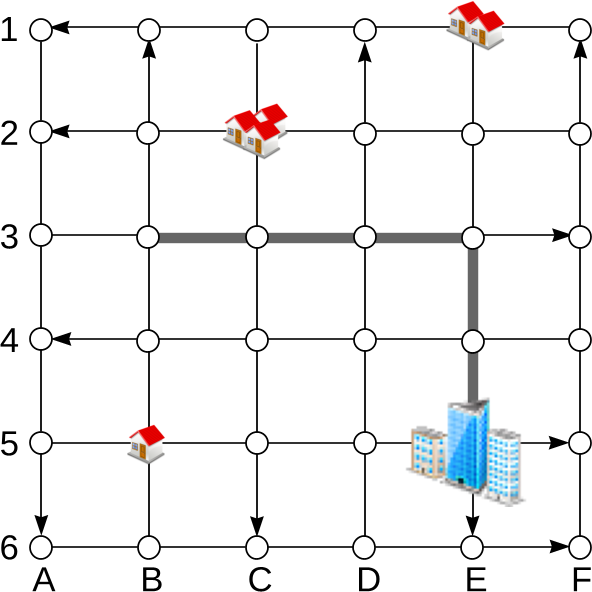
\includegraphics[width=7cm]{img/6x6grid.png}}
    \caption{Abstract grid scenario with the main origins (nodes B5, C2 and E1) and the main destination (node E5). Arrows show the links' directions. Thicker lines are the main links.}
    \label{fig:6x6grid}
\end{figure} 

The scenario settings are the same as in \cite{Bazzan+2008alamas}: every node is a possible origin or destination, although some nodes have higher probability of being an origin and one node has a high probability of being a destination. Table \ref{tab:odprob} shows the origins and destinations probability distribution, where PO means the probability of the node be an origin and PD is the probability of the node be a destination. With this feature, the scenario includes a real-world characteristic: the existence of main residential areas, where commuters depart from (nodes with higher chance of being origins) and a business center, where most commuters travel to (the node with high chance of being a destination).

{%
%\newcommand{\mc}[3]{\multicolumn{#1}{#2}{#3}}
\begin{table}[ht]
\begin{center}
\begin{tabular}{|l|c|c|} \hline
Node & PO & PD \\ \hline
E5 & 2.67\% & 60\% \\ \hline
B5 & 3\% & 1.15\% \\ \hline
C2 & 4\% & 1.15\% \\ \hline
E1 & 5\% & 1.15\% \\ \hline
Every other node & 2.67\% & 1.15\% \\ \hline
\end{tabular}
\caption{Origins and destinations probability distribution}\label{tab:odprob}
\end{center}
\end{table}
}%
%TODO INSTANTIATE Y AND Z
Regarding the road network capacity, there are main links, whose capacity is higher than the others, namely, 45 vehicles. The remaining links have the capacity of 15 vehicles. The main links are those between the nodes B3 to E3 and E3 to E5 (thicker lines on Fig. \ref{fig:6x6grid}). With this feature, the abstract 6x6 scenario becomes more realistic, as links' capacities are not homogeneous.

In the 6x6 grid scenario, 300 drivers populate the road network. Prior experimentation has shown that this number yields reasonable load in the road network. That is, with fewer drivers, congestions seldom occur and drivers don't need to look for alternative routes. On the other hand, with more drivers, most links get congested. This makes it difficult to assess the performance of the drivers because they have no attractive alternative routes.

The following metrics are evaluated in this scenario:

\begin{itemize}
  \item Number of aborted trips: this metric assesses how many drivers cannot find a path to their destinations within the limit of the learning episode (500 steps).
  \item Trip length: this metric assesses how many steps it takes for drivers to reach their destinations. If drivers take too many steps to finish their trips, this means that they are possibly building routes with loops.
 \item Travel time: this metric assesses how drivers' performance improve with time. More than just building a route without loops, drivers need to select links with low occupancy in order to achieve better travel times from their origins to their destinations.
\end{itemize}

\subsection{Nine OD pairs}
\label{sec:nineODDescription}
The abstract road network used in this scenario consists of 10 nodes and 24 links, as shown in Fig. \ref{fig:roadnetwork}. All nodes have 3 outbound links, except nodes 8, 9 and 10 which have 2, 1 and 0 outbound links respectively. Nodes 1, 2 and 3 are the possible origins and nodes 8, 9 and 10 are the possible destinations, resulting in nine possible OD pairs. All possible OD pairs have uniform probability of being assigned to a driver. %Table \ref{tab:routeEnum} shows the length and the number of shortest paths between the OD pairs, regarding the number of links between them.

% {%
% \begin{table}[ht]
% \begin{center}
% \begin{tabular}{|l|c|c|c|} \hline
% OD Pair & Shortest path length & Number of shortest paths \\ \hline
% 1-8 & 3 & 6 \\ \hline
% 1-9 & 3 & 3 \\ \hline
% 1-10 & 3 & 1 \\ \hline
% 2-8 & 2 & 1 \\ \hline
% 2-9 & 3 & 6 \\ \hline
% 2-10 & 3 & 3 \\ \hline
% 3-8 & 2 & 2 \\ \hline
% 3-9 & 2 & 1 \\ \hline
% 3-10 & 3 & 6 \\ \hline
% \end{tabular}
% \caption{Length and number of shortest paths for each OD pair in nine OD scenario}\label{tab:routeEnum}
% \end{center}
% \end{table}
% }%

Links' capacities are randomly assigned in the range [130:250] prior to the simulations. The values are persistent from one simulation to another to ensure a correct comparison of different approaches. The same is done for the amount of drivers on each OD pair. There are 1001 drivers on the road network. For Eq. \eqref{eq:tt}, $\fftt$ is set as 5 minutes for all links, $\tau = 1$ and $\beta = 2$ making travel time increase quadratically with the number of drivers. 

The choice of the range for the selection of links' capacities, the number of drivers and the parameters for Eq. \eqref{eq:tt} were made in this way to compare the results obtained in the present work with the ones obtained by the modified minority game for route choice \cite{Galib&Moser2011}.

% The range for 

\begin{figure}[ht]
    \centerline{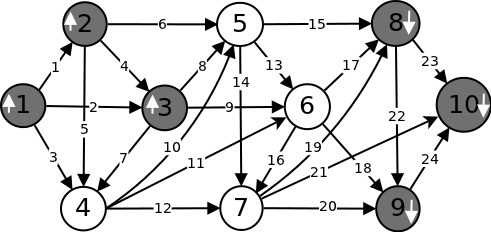
\includegraphics[width=8.5cm]{img/roadnetwork.png}}
    \caption{Road network, the same used by \cite{Galib&Moser2011}. Labels on links are identification numbers, nodes with upward arrows are the origins and downward arrows represent the destinations}
    \label{fig:roadnetwork}
\end{figure}

In this scenario, the RL for route choice approach is compared with three different route choice methods, as follows:

\begin{itemize}
  \item Random: At each step, drivers choose one of the possible outbound links with uniform probability.
  \item Greedy: At initialization, the shortest paths\footnote{It is possible to have more than one shortest path on the road network. Given that link's weights are equal, the shortest paths are the ones with less links.} for each driver are calculated. At each step, drivers choose one of the possible outbound links with a probability proportional to its capacity. The possible outbound links are the ones that belong to a shortest path. %TODO mention selfish here
  \item Minority Game: Drivers use the modified minority game approach proposed in \cite{Galib&Moser2011} to build their routes. A brief description of this approach is given in Section \ref{sec:related}. For a complete description, readers may refer to \cite{Galib&Moser2011}.
\end{itemize}

The comparison of the different route choice methods is based on metrics regarding the difference between expected and actual travel time as well as on road network load balance.

\subsubsection{Difference between expected and actual travel time:}
\label{sec:ttMetric}
In the real world, drivers have an expectation on the trip travel time, the expected load and the links' capacities. In the present work, for each driver $i$, the expected travel time $\ett{\optRoute{i}}$ on his shortest route $\optRoute{i}$ is given by Eq. \eqref{eq:ett}. In this equation, $\travTime$ is the travel time function defined in Eq. \eqref{eq:tt} applied to the estimated number of vehicles on the same route ($\expVeh{i}$). This estimation is given by the number of vehicles in driver $i$'s OD pair, plus a random number in the range $[-0,05 \times |D| : 0,05 \times |D|]$, where $|D|$ is the total number of drivers in the scenario. This ``noise'' is to simulate the effect of each driver ``guessing'' the number of vehicles going to the same destination.

\begin{equation}
\label{eq:ett}
\ett{\optRoute{i}} = \sum_{j \in \optRoute{i}}\travTime(\expVeh{i})
\end{equation}

In order to assess how reasonable the travel times obtained by drivers are, a metric called AED (\underline{a}ctual and \underline{e}xpected travel time \underline{d}ifference) was created. It is given by the average difference between actual and expected travel times of drivers in each OD pair. For this metric, negative values are preferred as this means that drivers are having lower travel times than expected. %It will be measured in terms of the mean and standard deviation of this difference for all drivers in a given OD pair. The mean will assess whether drivers are arriving at destination within their expectations, on average, and this happens when the metric reaches negative values (actual travel time is lower than expected). The standard deviation will evaluate whether there is a big difference between drivers' AED on the same OD pair, assessing the fairness of the route choice method.

\subsubsection{Road network load balance:}
\label{sec:loadBalanceMetrics}
From a global point of view, it is desired that vehicles get distributed proportionally to the capacity of each link in the network. When the number of vehicles ($\veh_j$) in a given link $j$ becomes greater its capacity ($\linkCap$), the link is congested. Road network load balance is measured in two forms: number of congested links ($n$) and average overload ($o$). Considering $C$ as the set of congested links, these metrics are measured according to Eq. \eqref{eq:balanceMetrics}. 

\begin{equation}
\label{eq:balanceMetrics}
\numCong = |\congRoads| \hspace{1.5cm}  \overLoadFactor = \frac{ \sum_{\substack{j \in \congRoads}} \left(\frac{\veh_j}{\linkCap} -1 \right)}{|C|}
\end{equation}

Both metrics are needed because $n$ alone does not measure how heavily the links are congested, while $o$ does not show how many links are overloaded. For both $n$ and $o$, lower values are preferred, as less links are congested and the severity of congestions is lower.

\section{Results and discussion}
\label{sec:results}

The following experiments have the goal of assessing the effect of Q-learning parameters, namely the learning rate ($\alpha$) and the discount rate for future rewards ($\gamma$) in both scenarios, so that these parameters can be adjusted accordingly. Plus, in the nine OD scenario, the RL approach is compared with the three route choice methods discussed in Section \ref{sec:nineODDescription}.

Experiment parameters' values are: for Eq. \eqref{eq:tt}, $\fftt$ is set as 5 minutes for all links, $\tau = 1$ and $\beta = 2$ making travel time increase quadratically with the number of drivers. Each execution consists of $\numepis = 100$ learning episodes. The initial and final values for the exploration coefficient are $\epsilon_0 = 1$ and $\epsilon_f = 0.01$, respectively. The value of the multiplicative factor that decreases $\epsilon$ is: $\lambda = \sqrt[100]{\frac{0.01}{1}} = 0.95499$.


\subsection{Q-learning parameters in the grid scenario}

%TODO do the alpha-gamma grid tests

In the grid scenario, the effect of Q-learning parameters was measured in terms of the number of aborted trips, the mean trip length and mean travel time for all drivers. In each execution (the repetition of $\numepis = 100$ episodes of the RL approach described in Section \ref{sec:proposal}), these values were registered and averaged over the last 10 episodes. For each parameter, 10 executions were made to generate the plots.

For the $\alpha$-varying tests, $\gamma$ was set as $1.0$ and for the $\gamma$-varying tests, $\alpha$ was set as $0.5$.

\begin{figure}
  \centering
  \subfigure[]{
    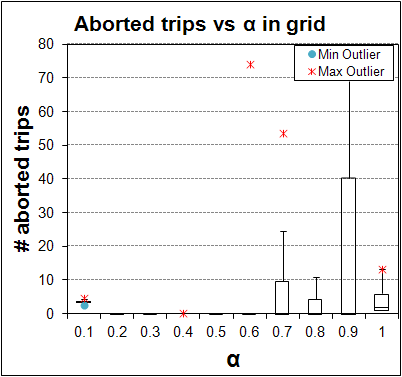
\includegraphics[width=6cm]{img/abortedTripsVsAlpha.png}
    \label{fig:abortedTripsVsAlpha}
  }
  \subfigure[]{
    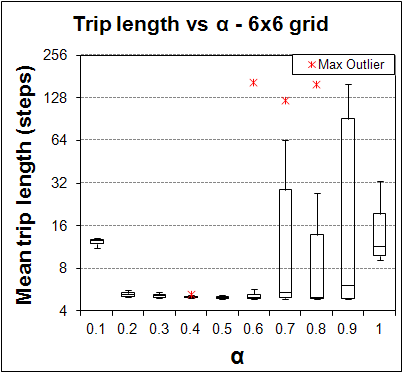
\includegraphics[width=6cm]{img/tripLengthVsAlpha.png}
    \label{fig:tripLengthVsAlpha}
  }
  \subfigure[]{
    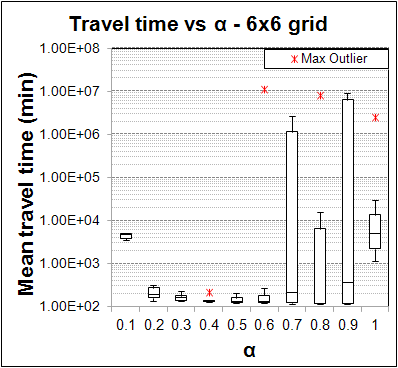
\includegraphics[width=6cm]{img/travelTimeVsAlpha-grid.png}
    \label{fig:travelTimeVsAlpha-grid}
  }
  \caption{Box-and-whisker charts showing the effect of $\alpha$ on the number of aborted trips \subref{fig:abortedTripsVsAlpha}, on the mean trip length \subref{fig:tripLengthVsAlpha} and on the mean travel time in log scale \subref{fig:travelTimeVsAlpha-grid} in the 6x6 grid scenario.}
  \label{fig:qLearningAlpha-grid}
\end{figure}

Figure \ref{fig:qLearningAlpha-grid} shows that, for high values of $\alpha$, drivers have poor performance as some of them do not manage to arrive at their destinations, increasing the number of aborted trips and the mean trip length. Also, travel times are very high. This shows that in a nonstationary scenario, a high learning rate is harmful.

\begin{figure}
  \centering
  \subfigure[]{
    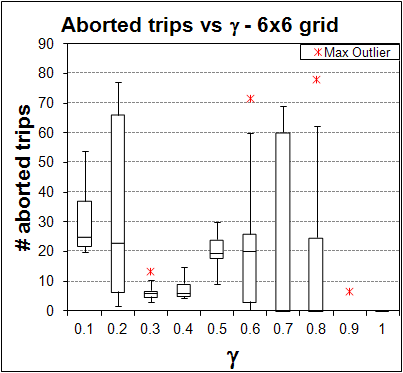
\includegraphics[width=6cm]{img/abortedTripsVsGamma.png}
    \label{fig:abortedTripsVsGamma}
  }
  \subfigure[]{
    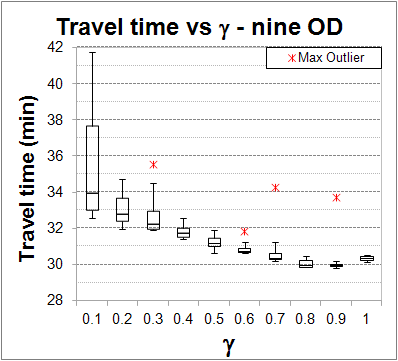
\includegraphics[width=6cm]{img/tripLengthVsGamma.png}
    \label{fig:tripLengthVsGamma}
  }
  \subfigure[]{
    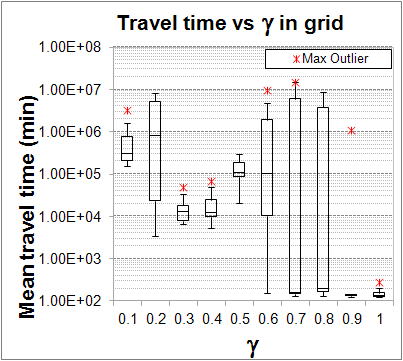
\includegraphics[width=6cm]{img/travelTimeVsGamma-grid.png} %TODO make it possible to see the zero
    \label{fig:travelTimeVsGamma-grid}
  }
  \caption{Box-and-whisker charts showing the effect of $\gamma$ on the number of aborted trips \subref{fig:abortedTripsVsGamma}, on the mean trip length \subref{fig:tripLengthVsGamma} and on the mean travel time in log scale \subref{fig:travelTimeVsGamma-grid} in the 6x6 grid scenario.}
  \label{fig:qLearningGamma-grid}
\end{figure}

Figure \ref{fig:qLearningGamma-grid} shows that the RL approach performs more robustly when $\gamma$ is high. For low values of $\gamma$, the interquartile range is large, which means that drivers are not learning the routes to their destinations or these routes have too many links. This shows that, in traffic scenarios, where the next choice options depend on the current, it is relevant to take into account the outcomes of the subsequent choices, otherwise the next available possibilities will result in a bad overall performance.

\subsection{Nine OD pairs scenario}

\subsubsection{Effect of Q-learning parameters:}
\label{sec:qlParamsNineOD}
In the nine OD scenario, the effect of Q-learning parameters was measured in terms of drivers' travel time. As this scenario has no loops and the number of possible routes is smaller than in the grid scenario, there is no need to evaluate the number of aborted trips and the mean trip length.

In each execution (the repetition of $\numepis = 100$ episodes of the RL approach described in Section \ref{sec:proposal}), the mean travel time for all drivers was registered and averaged over the last 10 episodes.  For each parameter, 10 executions were made to generate the plots displayed on Fig. \ref{fig:qLearningParams}.

\begin{figure}
  \centering
  \subfigure[]{
    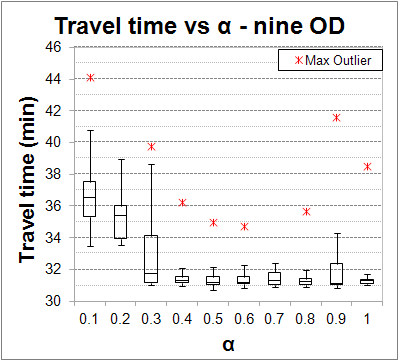
\includegraphics[width=6cm]{img/travelTimeVsAlpha.png}
    \label{fig:travelTimeVsAlpha}
  }
  \subfigure[]{
    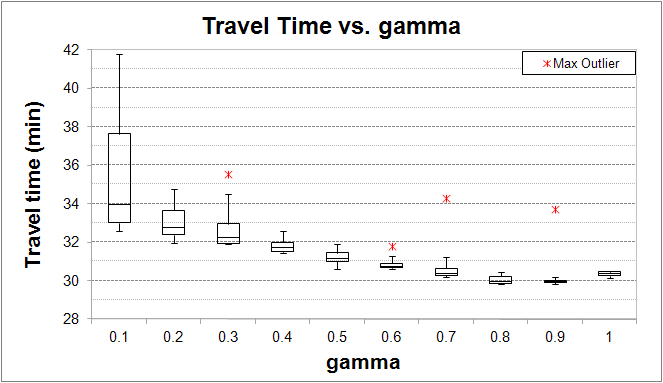
\includegraphics[width=6cm]{img/travelTimeVsGamma.png}
    \label{fig:travelTimeVsGamma}
  }
  \caption{Box-and-whisker charts showing the effect $\alpha$ and $\gamma$ on travel time in the nine OD pair scenario. Each parameter value was tested 10 times.}
  \label{fig:qLearningParams}
\end{figure}

Figure \ref{fig:travelTimeVsAlpha} shows that the approach performs robustly when $\alpha$ is within the range from 0.4 to 0.8, as the interquartile range is small.% For $\alpha = 1.0$ the interquartile range is the smallest, but the maximum outlier is too distant of the upper extreme. This can be due to the nonstationarity of the traffic scenario: if a driver disregards all the previous knowledge, the outcome of a single choice that brought bad results will be fully stored in the Q-table, so that the driver will not try it again (unless the action is tried again by exploration) even if the previous choices resulted in good outcomes. In this kind of nonstationary scenario, a high learning rate can lead to this effect.

Figure \ref{fig:travelTimeVsGamma} shows a decrease in the travel time when $\gamma$ is increased. For $\gamma = 0.9$, the smallest interquartile range and median are observed.

Analysing both scenarios, it is possible to see that the RL approach is less sensitive to the values of the Q-learning parameters in the nine OD scenario, because it is much simpler than the 6x6 grid in terms of the number of possible routes and the lack of returning links. 

\subsubsection{Comparison with other route choice methods:}
\label{sec:comparison}
In the following experiments, the goal is to compare the RL approach with the random, greedy and minority game (MG) approaches for route choice in the nine OD pairs scenario, as discussed in Section \ref{sec:nineODDescription}.

For the Q-learning update rule (Eq. \ref{eq:qlearning}) of the RL approach, $\alpha$ was set as 0.5 and $\gamma $ was set as 0.9 as these values resulted in good performance on the previous tests (Section \ref{sec:qlParamsNineOD}).

The AED metric (defined in Section \ref{sec:ttMetric}) for each approach is shown on Fig. \ref{fig:travelTimeComparison}. 

In this metric, the RL approach outperforms the others, as reasonable travel times (below drivers' expectation) are achieved in all OD Pairs. The minority game approach achieves travel times within expectation in four OD pairs. On the other OD pairs, the performance is still satisfactory, as actual travel times are no longer than five minutes beyond the expected, showing a degree of fairness of the approach. With the greedy method, drivers from five OD pairs have experienced travel times within expectation, but this approach has low fairness because, especially on OD pairs 1-10 and 2-8, actual travel times are far beyond the expected. The worst approach is the random, in which no drivers achieve reasonable travel times.

\begin{figure}[ht]
    \centerline{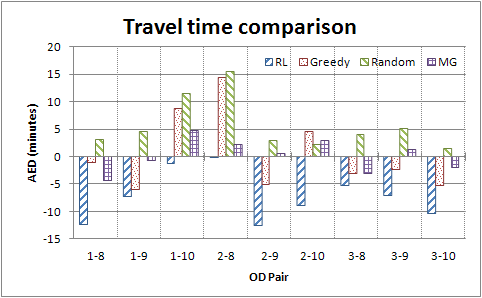
\includegraphics[width=10cm]{img/travelTimeComparison-hatched.png}}
    \caption{AED metric comparison for each route choice method. RL and MG are the reinforcement learning and minority game approaches, respectively}
    \label{fig:travelTimeComparison}
\end{figure}

\begin{figure}[ht]
  \centering
  \subfigure[]{
    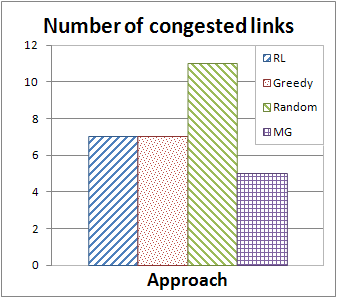
\includegraphics[width=5.8cm]{img/numCongestedRoads-hatched.png}
    \label{fig:numCongestedRoads} %TODO change order: RL / MG / (same as travel time)
  }
  \subfigure[]{
    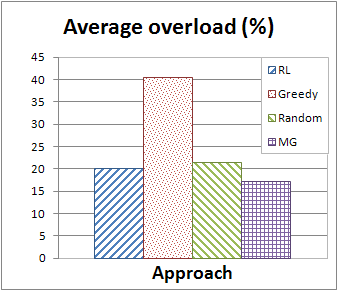
\includegraphics[width=5.8cm]{img/averageOverload-hatched.png}
    \label{fig:averageOverload}
  }
  \caption{Load balance evaluation in terms of number of congested links \subref{fig:numCongestedRoads} and the average overload \subref{fig:averageOverload}.}
  \label{fig:loadBalance}
\end{figure}




Using the load balance evaluation metrics defined in Section \ref{sec:loadBalanceMetrics}, Fig. \ref{fig:loadBalance} shows that the minority game based approach achieved the best result. Both the number of congested links and the average overload were the lowest. This means that vehicles were distributed over the network in a proportion that is closer to the links capacity. The better vehicle distribution explains why the achieved travel times are higher compared to the RL approach: minority game based drivers tend to avoid congested links even when these links would make the drivers arrive at their destinations faster than an uncongested alternative. 

The RL based approach achieves good results as the average overload shows that none of the seven congested links (out of 24 links) were heavily congested. Both the random and the greedy approach performed poorly, as many links were congested in the random approach and links were heavily congested in the greedy approach.



\section{Conclusions and future work}
\label{sec:conclusions}

In this work we modeled traffic assignment as a reinforcement learning problem and the driver agents were modeled as independent learners.

Using the proposed approach, drivers learned the routes between their origins and destinations in a reasonably complex grid scenario. Note that this is the case because cycles are possible thus the number of possible routes increases. Moreover, drivers learn how to build efficient routes, as the mean trip length and travel time reach lower values for certain parameters' values. In the grid scenario, the proposed approach has proven to be sensitive to the Q-learning update rule parameters. 

Especially when the learning rate is high, the learning process does not converge and several drivers do not find routes to their destinations. Also, the discount rate for future rewards must be high, otherwise drivers will not take into account the future consequences of the current choice, leading to bad options in the subsequent steps.

In the nine OD pairs scenario, our reinforcement learning approach for route choice was helpful in both the individual and the global points of view, as drivers achieve reasonable travel times (within expectation) on average, and traffic is distributed over the network, as links do not get heavily congested.

The RL approach outperformed the other route choice methods regarding drivers' experienced travel time. On average, drivers from all OD pairs achieved reasonable travel times, while the other methods did not achieve this.

%In terms of load distribution over the road network, the proposed RL approach was slightly outperformed by the minority game based approach proposed by \cite{Galib&Moser2011}. 

The proposed approach has the advantage of making realistic assumptions as it only relies on drivers' own experience about the road network (i.e. the experienced travel time). This way, the use of real-time information and historical data of links is not necessary. This makes our approach an attractive and feasible alternative to be used on existing navigation systems, as no new technology is required. That is, as navigation systems are already capable of recording travel time for traversing a given road, the RL approach can be helpful as this is the only information it needs.

Further investigation can be conducted to evaluate scenarios with heterogeneous drivers. It would be interesting to investigate whether the RL drivers can adapt themselves to the greedy drivers or even the ones using the minority game approach proposed by \cite{Galib&Moser2011}. Future work can also attempt to investigate joint action learning mechanisms for this transportation domain. %TODO further microscopic investigation 

\section*{Acknowledgments}

Authors would like to thank the anonymous reviewers for their careful review and helpful suggestions of paper improvements as well as Mr. Syed Galib for clarifying questions on the minority game for route choice approach and for providing data for comparison. Both authors are partially supported by CNPq (project LabTrans, scholarship and research grant) and FAPERGS (project RS-SOC). %The authors also would like to thank the anonymous reviewers for their suggestions of paper improvements.

\bibliographystyle{plain}
\bibliography{references,stringDefs,AB,CD,EG,HJ,KL,MO,OURS,PR,S,TZ} 

\end{document}
